\chapter{Methods for solving QUBO problems}\label{review}
\vspace{2em}

This chapter reviews the different approaches used to solve QUBO problems. They can be broadly categorised as Classical, Quantum Annealing, Neural Network Quantum States, and Hybrid Quantum-Classical Algorithms.

\section{Classical}
Classical approaches search for solutions to QUBO problems without exploiting quantum properties. A typical classical approach is by exact diagonalisation of the corresponding Ising Hamiltonian~\cite{b25}. Exact diagonalisation solves for all the eigenvalues and eigenvectors and is also known as eigendecomposition, which is always possible for quantum Hamiltonians as they are represented by Hermitian matrices~\cite{b27}. However, the runtime of exact diagonalisation scales exponentially with input problem size and becomes computationally infeasible once the matrix grows large \cite{b25}. Since we are only interested in finding the smallest eigenvalue and the corresponding eigenvector, we can use iterative methods such as the Lanczos algorithm or the implicitly restarted Arnoldi method to find the smallest eigenvalue~\cite{b28,b29}. However, such methods also often run into stability issues. There are also branch and bound methods for solving QUBO problems, which aim to break down the QUBO into subproblems and build lower and upper bounds for the objective values \cite{otaki2023experimental}. However, such methods are often built for specific classes of problems and may not apply to a general QUBO problem.

Due to the exponentially increasing search space, some classical methods aim to find approximate solutions to QUBO problems instead. One class of such methods relies on "heuristics" to search for optimal solutions~\cite{b12}. Dunning et al.\yrcite{b12} systematically reviewed and evaluated published heuristics for QUBO problems. However, heuristics often only work well for some QUBO problems and do not generalise well.

%For example, variants of Tabu search---a local search algorithm that allows for moves that are not improvements and discourages visiting already visited states---are highly competitive heuristic algorithms to find good solutions to QUBO problems\cite{b2,b30}. 

Another classical approximate method for solving QUBO problems is simulated annealing (SA). Simulated annealing \cite{Kirkpatrick} is a probabilistic method that starts with an initial trial state and a temperature $T$, which decreases slowly during the search. In each iteration, the algorithm samples neighbouring states of the current state and accepts the new sample based on the difference in energy, $\Delta E$, between the current state and the new state. If $\Delta E < 0$, then the new sample is always accepted, and if $\Delta E \geq 0$, the new sample is accepted with a probability $\propto e^{-\frac{\Delta E}{T}}$. The algorithm to sample new states is adapted from the Metropolis-Hastings sampling method \cite{metropolissampling}, and the chance to explore poorer solutions allows the algorithm to escape local minima.

There are various classical approaches to solving QUBO problems, as they have been studied extensively. For a detailed survey of classical methods for solving QUBO problems, refer to \cite{punnen2022quadratic}.

\section{Quantum Annealing}\label{section:annealing}
Quantum annealing, introduced by Kadowaki and Nishimori \yrcite{kadowaki1998quantum}, finds the ground state configuration of Ising models. For a QUBO problem, we convert it to the equivalent Ising model and then use the \textit{adiabatic theorem} to find its ground state configuration. The \textit{adiabatic theorem} states that "a quantum system in its ground state will remain in the ground state, provided that the Hamiltonian governing the dynamics changes sufficiently slowly" \cite{b14,b15}. Suppose we can manipulate the final Hamiltonian of a quantum system to one that describes the Ising model of interest. In that case, we can find the ground state of the Ising model simply by measuring the final configuration of the quantum system.

\begin{figure}[h!]
    \centering
    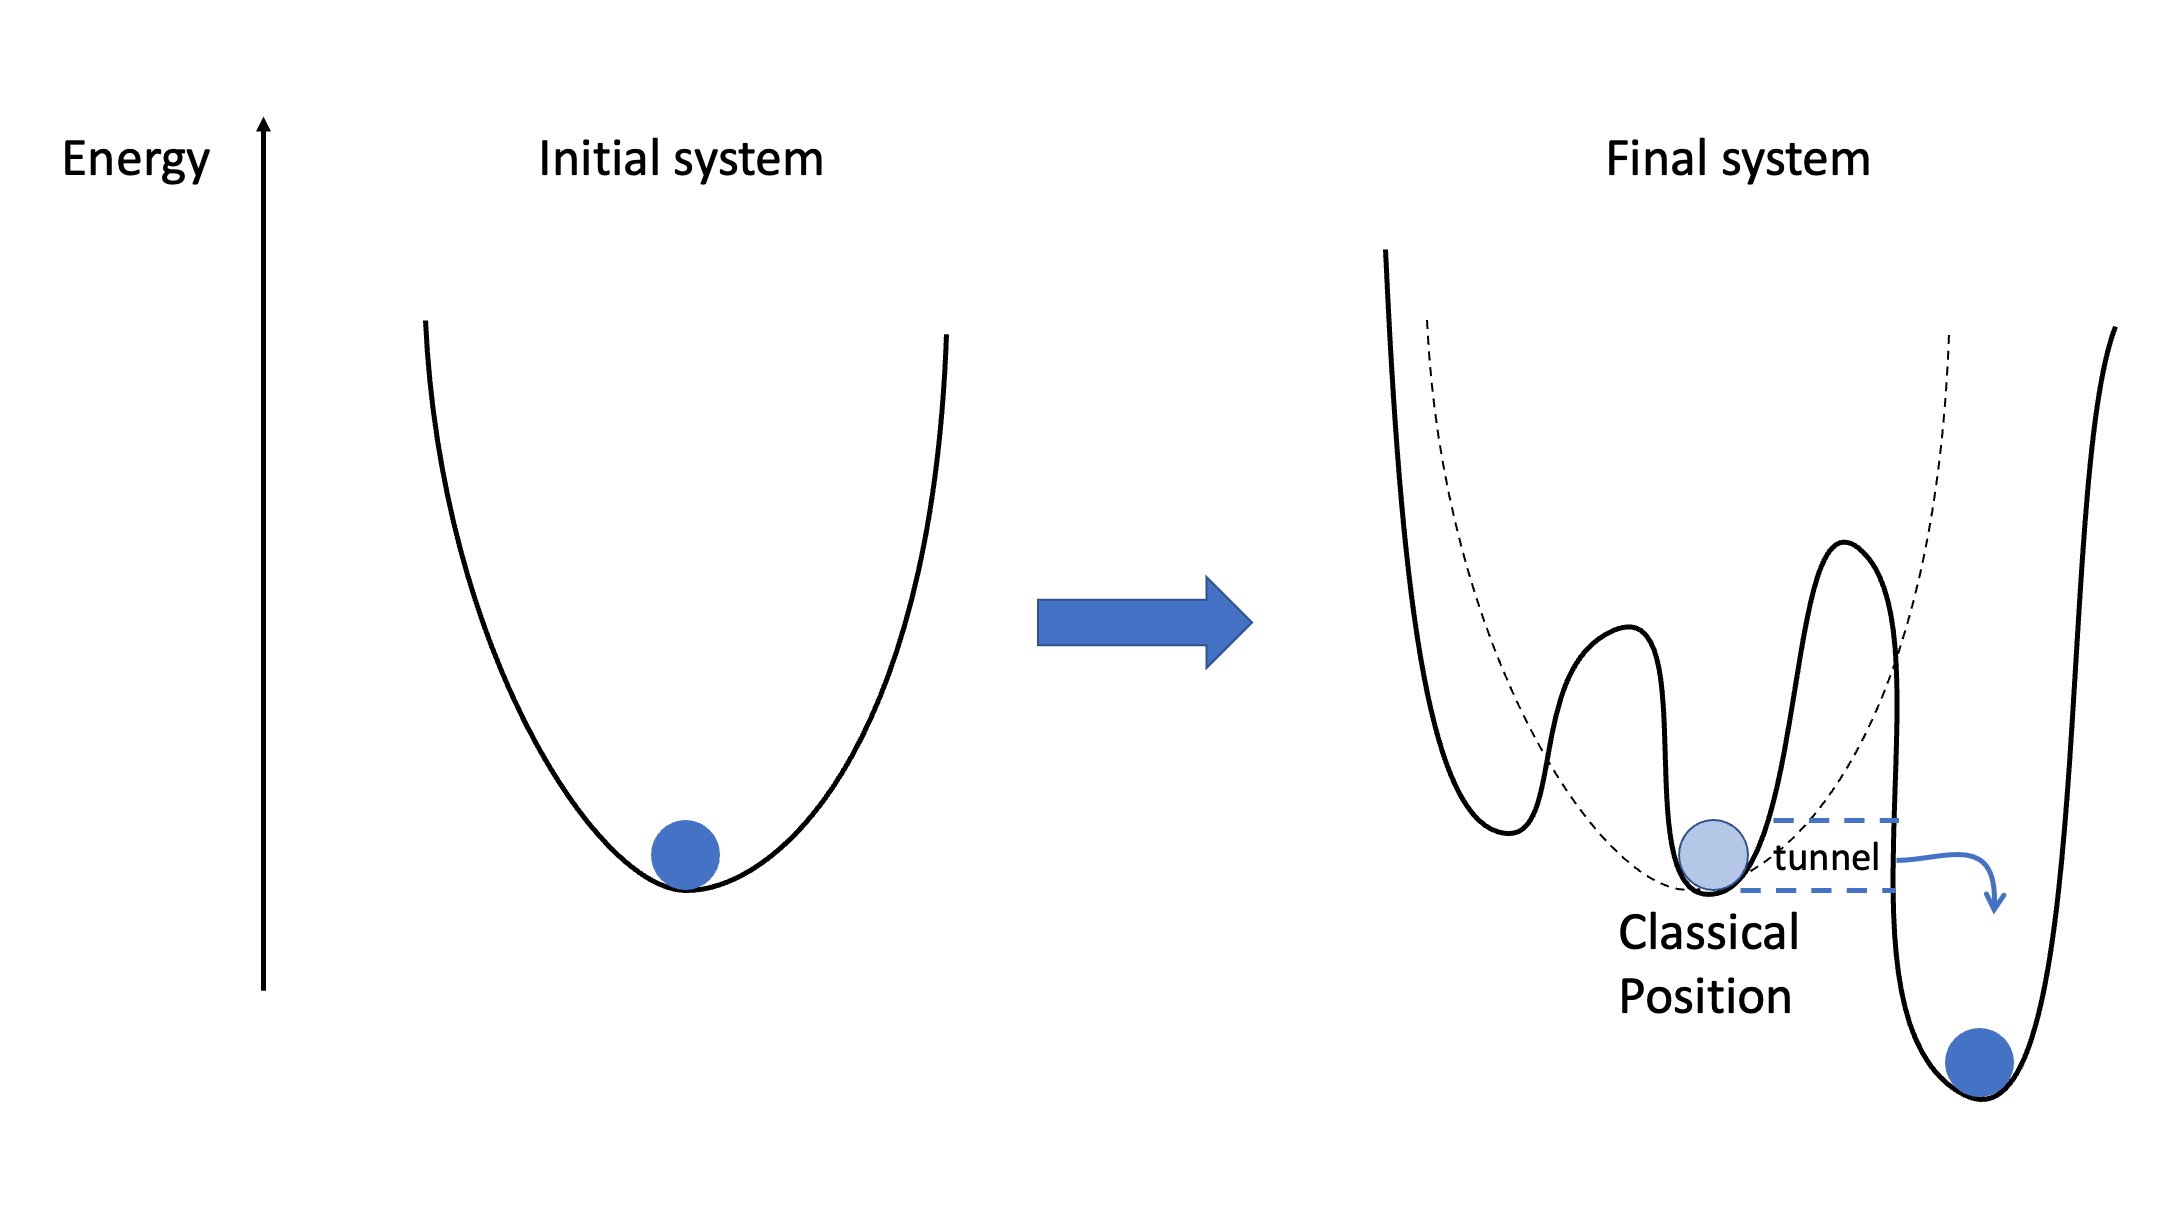
\includegraphics[width=0.8\linewidth]{images/quantum_annealing.png}
    \caption{Energy landscape before (left) and after (right) quantum annealing}
    \label{quantumannealing}
\end{figure}
Quantum annealers first prepare a system in the ground state with a simple initial Hamiltonian $H_0$ (called the mixer or tunnelling Hamiltonian), with a simple energy landscape on the left of \autoref{quantumannealing}. Then, the system Hamiltonian is slowly changed to a more complex form $H_c$ \cite{b10}, with a complex energy landscape on the right of \autoref{quantumannealing}. The Hamiltonian at any point $H(s)$ can be written as
\begin{equation}
    \label{eqn:annealinghamiltonian}
    H(s) = A(s)H_0 + B(s)H_c
\end{equation}
where $s \in [0,1]$ is the normalised anneal fraction and $A(s)$ and $B(s)$ are decreasing and increasing functions. At the start of the annealing, we should have $A(s) >> B(s)$, and at the end of the annealing, we should have $B(s) >> A(s)$. If the transition time is sufficiently large, the adiabatic theorem ensures that the system will remain in the ground state, which can then be measured to yield the desired ground state configuration of $H_c$ \cite{b14}. 

As $H_0$ usually consists of a transverse magnetic field and does not commute with the target Hamiltonian $H_c$, it allows for quantum tunnelling effects through energy barriers between classical states \cite{kadowaki1998quantum}. Quantum effects allow the wave function to remain at the ground state even when classical search methods may end up stuck in a local minimum. However, the adiabatic theorem requires an arbitrarily long anneal time to guarantee that the system remains in the ground state, which is not feasible for practical purposes. Current implementations of quantum annealing instead rely on a finite time approximation with repeated sampling to increase the success rate \cite{farhi2001}.

Quantum annealing has been extensively studied and applied to solve many problems, such as scheduling problems \cite{b17}, portfolio optimisation \cite{b18}, and quantum simulations \cite{b19}. Even though there are significant roadblocks in scaling the currently limited hardware capabilities \cite{b14}, with debate on whether quantum annealing will eventually run faster than classical search methods \cite{b10}, there is hope that these challenges can be tackled soon with the rapid progress made in quantum computing technology. D-wave is the current leading commercial provider of quantum annealing hardware \cite{b16}.

\section{Neural-Network Quantum States}
Carleo and Troyer \cite{b20} introduced a neural-network-based method for modelling the wave function of a target quantum system known as \textit{neural-network quantum states} (NNQS). The authors used the approach to find the ground state and time evolution of the Ising and Heisenberg models in Physics. The NNQS is used as an Ansatz to approximate the wave function, which can be viewed as a probability distribution of a system \cite{b25}. The more general method of using an Ansatz as a trial wave function and minimising its energy through Monte Carlo sampling is also known as variational Monte Carlo.

The theoretical foundations for NNQS to approximate wave functions of quantum systems rely on the Kolmogorov–Arnold representation theorem \cite{kolmogorov1957representation}, which implies that neural networks can represent all multivariate, smooth functions. Since the wave function generally satisfies these requirements, we can expect that a neural network can reasonably approximate the wave function of a quantum system \cite{b20}.

The original NNQS architecture utilised a Restricted Boltzmann Machine (RBM) as its neural network \cite{b20}. The RBM, shown in \autoref{rbmstructure}, is an energy-based generative model that has three components: a visible layer $\boldsymbol{s}$ with $n$ nodes, a hidden layer $\boldsymbol{h}$ with $m$ nodes, and a weight matrix $\mathbf{W}$. The number of hidden nodes is generally a multiple of the number of visible nodes, and the ratio $\alpha = \frac{m}{n}$ is a hyperparameter of the model. Each visible node $s_i$ is connected to every hidden node $h_j$ with a certain weight $W_{ij}$, but there are no connections within the visible or hidden layer. In other words, the visible and hidden nodes of the RBM form a bipartite graph.
\begin{figure}[h!]
    \centering
    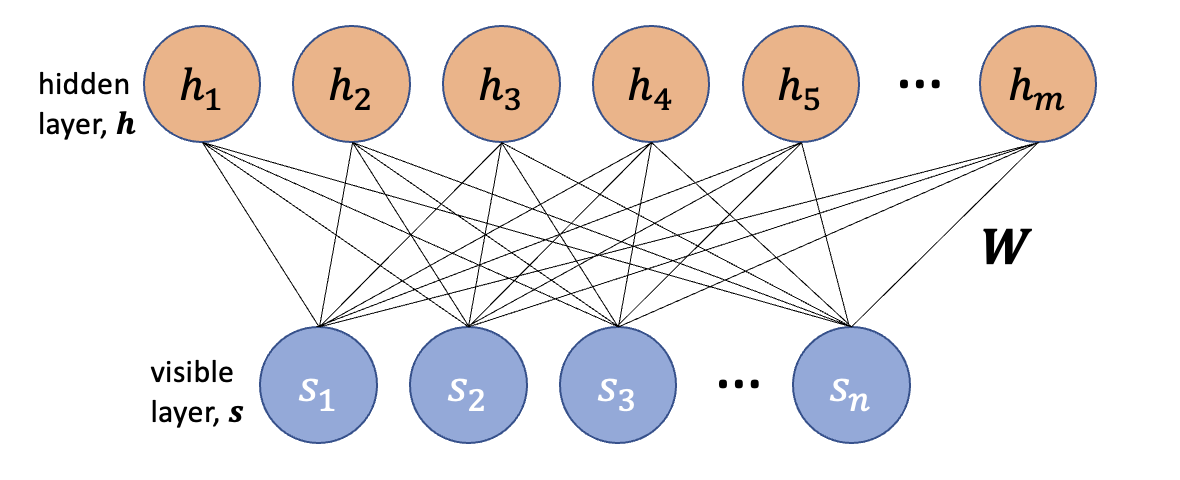
\includegraphics[width=0.9\linewidth]{images/rbm_diagram.png}
    \caption{Structure of Restricted Boltzmann Machine}
    \label{rbmstructure}
\end{figure}

When approximating the wave function of an Ising model, each visible node $s_i$ represents the spin of a particle in the Ising model and can only take on the values of $1$ and $-1$ \cite{b20}. The representation of the wave function by the RBM can be expressed as:
\begin{equation}
    \Hat{\Psi}(\boldsymbol{s} ; \boldsymbol{\theta}_{rbm}) = \sum_{h} e^{\sum_i a_s s_i + \sum_j b_j h_j + \sum_{i,j}W_i s_i h_j} 
\end{equation}
where  $\boldsymbol{\theta}_{rbm} = \{\boldsymbol{a}, \boldsymbol{b}, \boldsymbol{W}\}$ are the biases and weights of the RBM \cite{b20}. The network weights $\mathbf{W}$ are usually updated by performing Gibbs sampling, calculating the average energy of sampled configurations, and using gradient-based optimisers or the stochastic reconfiguration method to derive weight updates \cite{b25}.

Other neural network architectures, such as the Multilayer Perceptron (MLP), can also be used for NNQS. An MLP model is a feedforward artificial neural network that consists of an input layer $\boldsymbol{x}$, one or more hidden layers, and an output layer. Each layer is fully connected to the next layer with certain weights, and each node has a non-linear activation function $\sigma$ such as the sigmoid or ReLU function. 

\begin{figure}[h!]
    \centering
    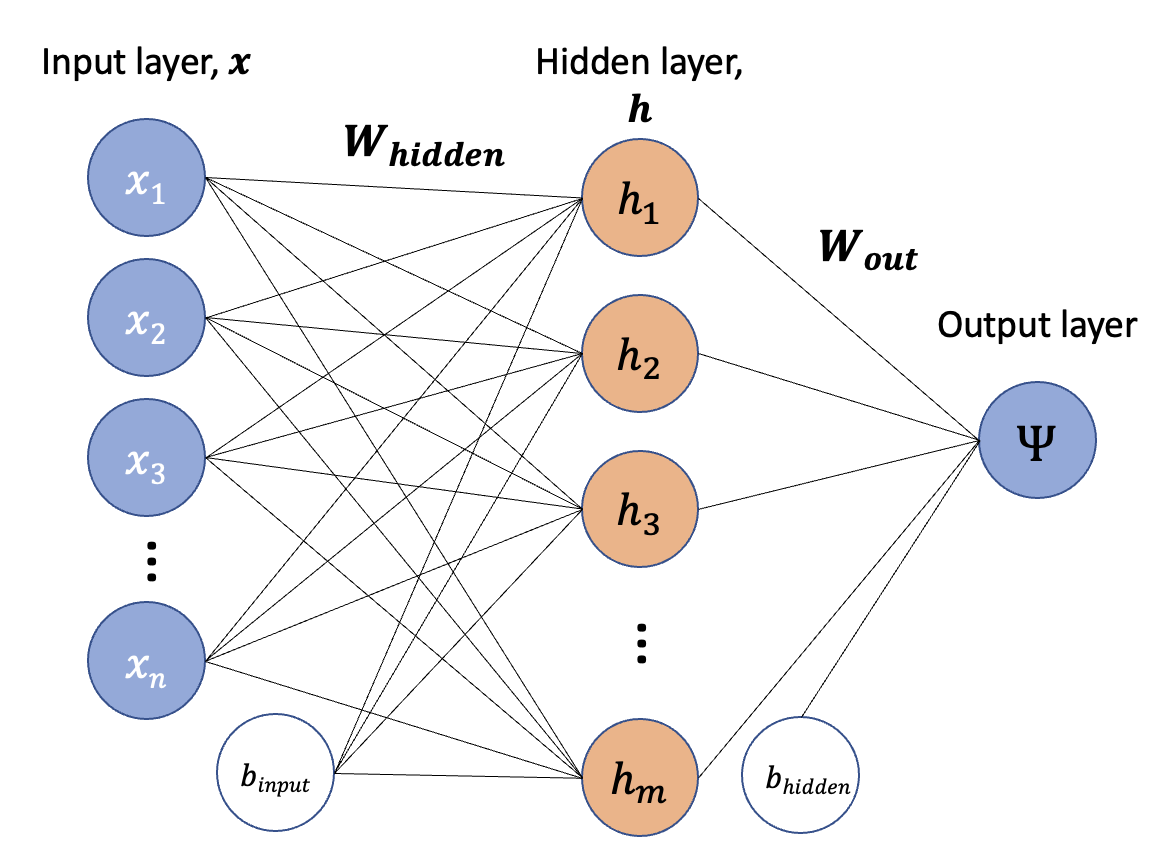
\includegraphics[width=0.7\linewidth]{images/mlp_diagram.png}
    \caption{Structure of Multilayer Perceptron with one hidden layer and one real-valued output node}
    \label{rbmstructure}
\end{figure}
When approximating the wave function of an Ising model, each input node $x_i$ represents the spin of a particle in the Ising model, and the output nodes represent the value of the wave function. If we assume the wave function to be real and positive, then only one output node is needed to represent the real part of the wave function \cite{b20}. With a complex wave function, we could use two output nodes that represent the real and imaginary components of the wave function. With one hidden layer, the MLP representation of the wave function can be expressed as:
\begin{equation}
    \Hat{\Psi}(\boldsymbol{x}; \boldsymbol{\theta}_{mlp}) = 
    \sigma_{out} \left(
    \boldsymbol{W}_{out} \hspace{2px}
    \sigma_{hidden} \left( \boldsymbol{W}_{hidden}\boldsymbol{x} + \boldsymbol{b}_{input} \right) + \boldsymbol{b}_{hidden} \right)
\end{equation}
where  $\boldsymbol{\theta}_{mlp} = \{\boldsymbol{W}_{hidden}, \boldsymbol{b}_{input}, \boldsymbol{W}_{out}, \boldsymbol{b}_{hidden}\}$ are the weights and bias of the MLP and $\sigma_{out}, \sigma_{hidden}$ are the non-linear activation functions of the nodes \cite{b20}. The MLP is trained similarly to the RBM, except that a more general sampling method, the Metropolis-Hasting algorithm, is used \cite{b25}.

\section{Hybrid quantum-classical}
Hybrid quantum-classical methods are designed to use current limited quantum computing resources by integrating them with classical optimisers to solve QUBO problems \cite{b32}. One such algorithm is the Quantum Approximate Optimization Algorithm (QAOA) \cite{b23}. Like NNQS, QAOA aims to find an approximation of the ground state of an input Hamiltonian using an Ansatz. The Ansatz used is a gate-based quantum circuit with $2p$ variational parameters $\gamma_1, \beta_1, \ldots, \gamma_p, \beta_p$ optimised with a classical optimiser \cite{b34}. For a problem size $n$. the algorithm first prepares a quantum state $| + \rangle^{\otimes n}$ in uniform superposition by applying the Hadamard gate to $n$ qubits. The trial wave function is then constructed with:
\begin{gather}
    \Hat{\Psi}(\boldsymbol{\gamma}, \boldsymbol{\beta}) = U_B(\beta_p) U_C(\gamma_p)...U_B(\beta_1) U_C(\gamma_1) | + \rangle^{\otimes n} \\
    U_C(\gamma) = e^{-i\gamma H_c} \\
    U_B(\beta) = e^{-i\beta H_0}
\end{gather}
Using the time-independent Schrödinger equation, we can see that $U_c$ and $U_B$ are operators that evolve the state with the Hamiltonian $H_c$ (problem Hamiltonian) and $H_0$ (an easy-to-implement, mixing Hamiltonian) for time intervals $\boldsymbol{\gamma}$ and $\boldsymbol{\beta}$. At the same time, the parameter $p$ determines the number of time evolutions of the final state \cite{b34}.

Each operation in the mixing Hamiltonian is implemented with a single rotation gate $R_X$ while the two-qubit operations in the problem Hamiltonian are implemented with a 2-qubit $R_{ZZ}$ gate \cite{qaoareview}. A circuit diagram of the QAOA circuit is shown in \autoref{qaoacircuit} with the Hadamard gates on the left, repeated blocks of $U_c$ and $U_B$ operators and a measurement of the final qubit states. The state is then measured repeatedly to obtain samples of the qubit configurations, the energies of the samples are calculated, and $\boldsymbol{\gamma}$ and $\boldsymbol{\beta}$ are optimised to minimise the average energy of the samples. The final solution can be determined by repeatedly sampling from the trial wave function with the optimised parameters.

\begin{figure}[h!]
    \centering
    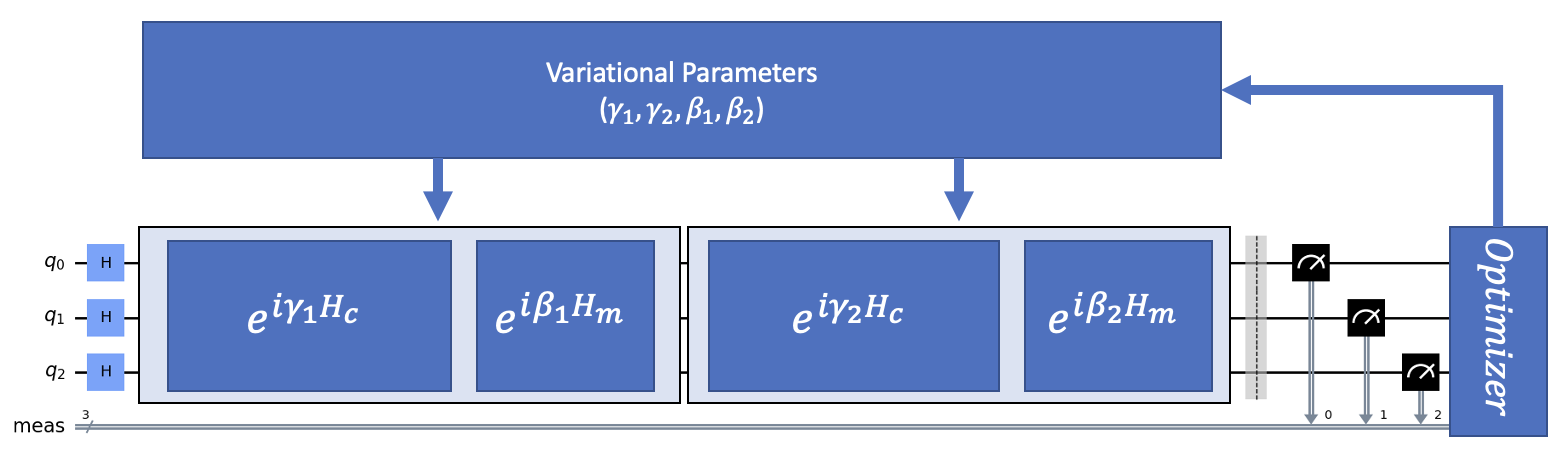
\includegraphics[width=\linewidth]{images/qaoa_circuit.png}
    \caption{Circuit diagram of the QAOA algorithm circuit with $p=1$}
    \label{qaoacircuit}
\end{figure}

QAOA can be regarded as a discretised version of Quantum Annealing \cite{qaoareview}. There is evidence that QAOA is more difficult for classical computers to simulate than Quantum Annealing, which may suggest that it could be a better way to demonstrate quantum supremacy \cite{farhi2016quantum}. In the noisy intermediate-scale quantum (NISQ) era, quantum computers are not yet stable enough to reliably run deep and complex quantum circuits \cite{qaoareview}. Hybrid methods could serve as the intermediate solution for optimisation problems on quantum computers. In contrast to quantum annealing, which can only be run on specialised quantum annealing devices, QAOA can be implemented on a general gate-based quantum computer \cite{b22}. 